\subsection{Introduction to linear systems}

A linear system can be written as
$$ \mat{A}\vec{x} = \vec{b} $$
where $\mat{A}$ is a  matrix of size $m \times n$ (we suppose $m \geq n$) and $\vec{x}$ is a coulumn  vector of length $n$  and $\vec{b}$ is  a column vectors of length $m$. $\vec{x}$ represents the unknown solution while $\vec{b}$ is a given vector. This form can be expanded as
$$
    \begin{matrix}
        a_{11}x_1 + a_{12}x_2 + \hdots + a_{1n}x_n = b_1\\
        a_{21}x_1 + a_{22}x_2 + \hdots + a_{2n}x_n = b_2\\
        \vdots\\
        a_{m1}x_1 + a_{m2}x_2 + \hdots + a_{mn}x_n = b_m
    \end{matrix}
$$

We are interested in:

\begin{itemize}
    \item Existence and uniqueness of a solution
    \item Numerical methods to find the solution
    \item Conditioning of the problem
\end{itemize}

We separately consider the case of square linear systems ($m=n$) and leasst squares problem ($m>n$).

\subsection{Square linear systems}


\begin{proposition}
    The solution of a linear system
    $$ \mat{A}\vec{x} = \vec{b} $$
    with $\mat{A}$ of dimension $n \times n$, $\vec{x}$ and $\vec{b}$ of dimension $n$ exists and is unique iff one of the following conditions holds:
    
    \begin{itemize}
        \item $\mat{A}$ is non-singular
        \item $\rank{A} = n$
           \item  The system $\mat{A}\vec{x} = \vec{0}$ admits only the solution $\vec{x} = \vec{0}$
    \end{itemize}

\end{proposition}

The solution can be algebraically computed in the following way
$$ \mat{A}\vec{x} = \vec{b} \implies \inv{A}\mat{A}\vec{x} = \inv{A}\vec{b} \implies \vec{x} = \inv{A}\vec{b} $$
The problem with this kind of method is that computing the inverse of $\mat{A}$ can be expensive for large values of $n$.

Another method to compute the solution of a system is \textit{Cramer's rule}:
$$ x_i = \frac{\det{A_i}}{\det{A}},\ i = 1, \hdots, n $$
where $\mat{A}_i$ is obtained from $\mat{A}$ by replacing the $i$-th column by $\vec{b}$

As for the previous one, the computation of determinants can be quite expensive for large values of $n$.

We will consider two different approaches to find the solution of a linear system:

\begin{itemize}
    \item \textit{direct methods}. They yield the solution in a finite number of steps; they are more precise but more expensive in terms of computational cost
    \item \textit{iterative methods}. They require (in principle) an infinite number of steps; they are less precise and less expensive
\end{itemize}

It is very important to perform also an error analysis on the  obtained results.  It generally includes two parts:
\begin{itemize}
    \item \em{Rounding} or \em{arithmetic errors}. They depend on the algorithm steps. An algorithm producing an arithmetic error limited by a constant is called a \textbf{stable algorithm}.
    \item \textit{Inherent errors}. They are due to the errors in the data representation and the DO NOT depend on the algorithm. For this reason, if the inherent error is large,we speak about  \textbf{ill-posed problem}.
\end{itemize}

\subsection{Direct methods}

In the case of direct methods we factorize the matrix A as in section \ref{sec:matdecomp}.
Let $\mat{A}=\mat{L} \mat{U}$  , then 
 the solution of the linear system $\mat{A}\vec{x} = \vec{b}$ can be computed by solving two triangular systems
$$
    \begin{matrix}
        \mat{L}\vec{y} = \vec{b}\ \text{(forward substitutions algorithm)}\\
        \mat{U}\vec{x} = \vec{y}\ \text{(backward substitutions algorithm)}
    \end{matrix}
$$

\textbf{Forward substitution.}

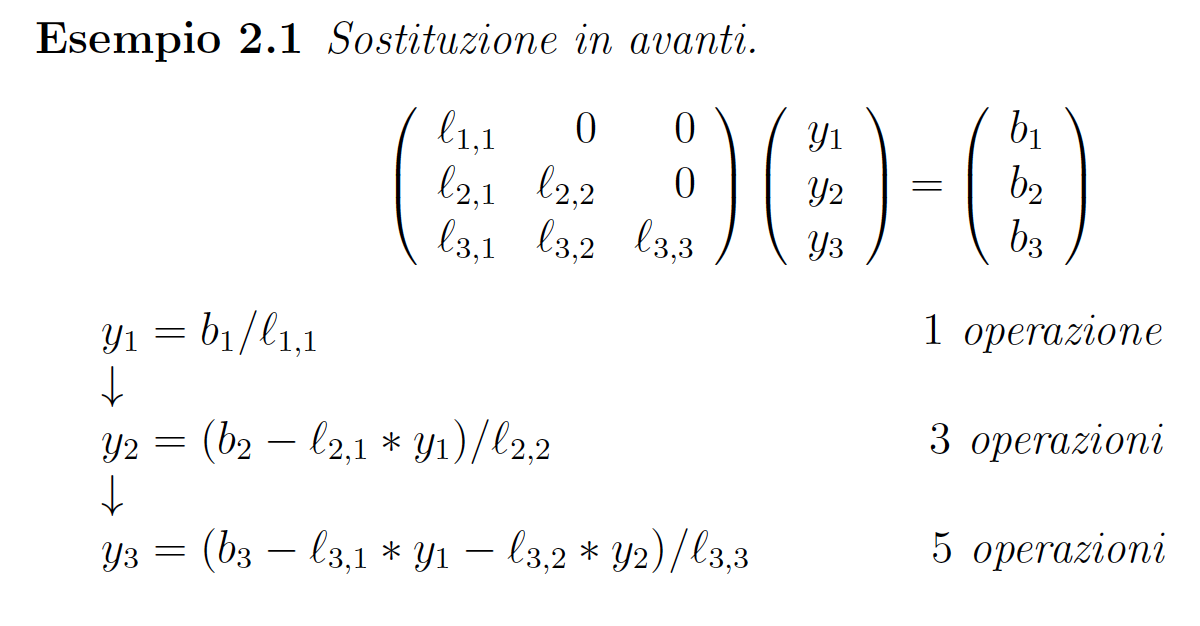
\includegraphics[width=0.7 \textwidth]{sections/images/forsub.png}

\textbf{Backward substitution.}

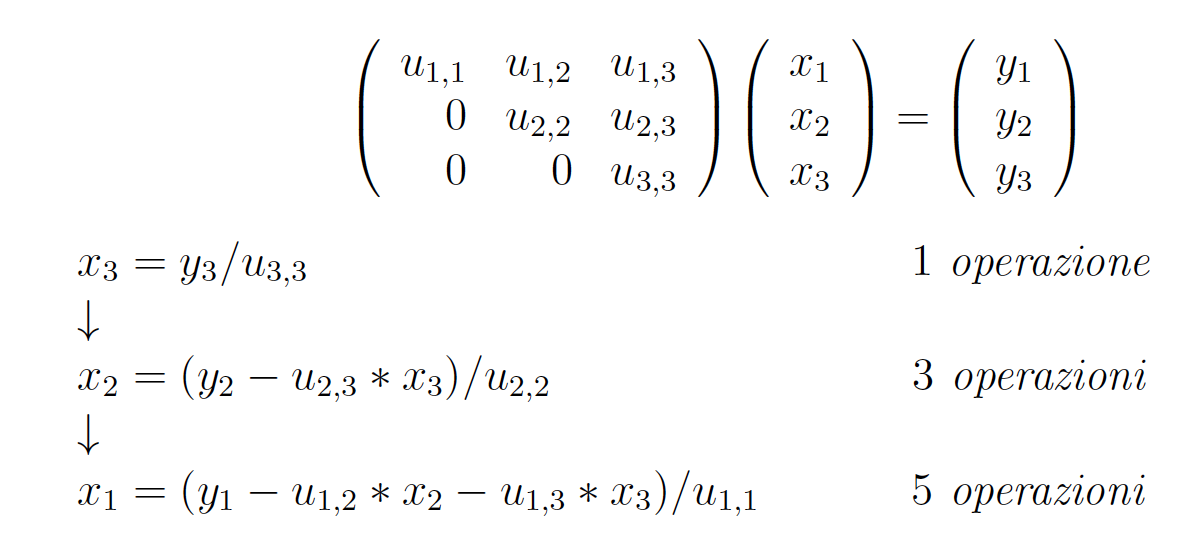
\includegraphics[width=0.7 \textwidth]{sections/images/backsub.png}

In the case of pivoting algorithm, we have that  $\mat{P} \mat{A}=\mat{L} \mat{U}$. Then 
 the solution of the linear system $\mat{P} \mat{A}\vec{x} = \mat{P} \vec{b}$ can be computed by solving two triangular systems
$$
    \begin{matrix}
        \mat{L}\vec{y} = \mat{P}\vec{b}\ \text{(forward substitutions algorithm)}\\
        \mat{U}\vec{x} = \vec{y}\ \text{(backward substitutions algorithm)}
    \end{matrix}
$$

\subsection{Iterative methods}

Iterative methods are numerical methods that approximate a solution using a procedure involving several (or an infinite amount of) steps. 
%Each iteration requires $n^2$ multiplications, meaning that these methods have a computational cost of $\mathrm{O}(n^2)$.

The basic idea of iterative methods is to construct a sequence of vectors $\vec{x}_k$  enjoying the property of \textit{convergence}
$$ \vec{x}^* = \lim_{k \rightarrow \inf}{\vec{x}_k} $$
where $\vec{x}^*$ is the exact solution and the starting guess $\vec{x}_0$ is given.

In general the sequence $\vec{x}_k$ is obtained as $\vec{x}_k=g(\vec{x}_{k-1}), \ k=1,\ldots$ where $g$ is a particular function or set of operations acting on $\vec{x}_{k-1}$.
Different classes of iterative methods are defined for different expressions of $g$.
In general, an iterative method converges for matrices with fixed properties (such as on the shape, on the eigenvalues, ...).

Iterative methods are sensitive to both algorithmic and truncation errors.

Examples of iterative methods (the most common):

\begin{itemize}
    \item \textit{stationary iterative methods}, they take the form
    $$\vec{x}_{k+1} = \mat{B}\vec{x}_k + \vec{f}$$
    where $\mat{B}$ is called \textit{iteration matrix} and $\vec{f}$ is a vector obtained from $\vec{b}$
    \item \textit{gradient-like methods}, they take the form
    $$\vec{x}_{k+1} = \vec{x}_k + \alpha_k\vec{p}_k$$
    where $\alpha_k \in \set{R}$, $\vec{p}_k$ is a vector called \textit{direction}.
    
    If $\mat{A}$ is symmetric and positive definite and the vectors $\vec{p_k}$ have the \textit{conjugacy} property, i.e:
    $$\vec{p}_i^T\mat{A}\vec{p}_k=0 \ \ if \ i \neq k $$
    then the method is called \textit{Conjugate Gradients}.
\end{itemize}

All these methods require one matrix-vector multiplication per iteration. Hence, if $\mat{A}$ is a \textit{full} matrix the computational complexity is $O(n^2)$  per iteration.

Stopping criteria for iterative methods for linear systems are:
\begin{itemize}
\item defined the residual $\vec{r}_k=\bb-\AAA\xx_k$ at iteration $k$, stop the algorithm when
\begin{itemize}
   \item $\|\vec{r}_k\| \le \epsilon$ (absolute criterion)
    \item $\frac{\|\vec{r}_k\|}{\|\bb\|} \le \epsilon$ (relative criterion)
    \end{itemize}
    \item $\|\vec{x}_{k+1}-\vec{x}_k\| \le \tau$ (absolute criterion)
\end{itemize}

\textbf{Sparse matrices}
A matrix $\mat{A}$ is called \textit{sparse} if it has a very small percentage (i.e. $0.05-0.06 \%$ ) of non-null elements. In this case, the matrix is not fully stored, but only the non-null elements and their indices are stored. The matrix-vector multiplication requires $k$ multiplications, where $k$ is the number of non-null elements.


\subsection{Inherent errors in linear systems}
WE remind that inherent errors are due to the errors in the data representation. They \textbf{do not} depend on the algorithm used for computing the result. Really, the analysis of inherent errors is performed by supposing to use exact arithmetic to  compute the result. 

Consider now a linear system $\mat{A}\vec{x} = \vec{b}$. What happens to the solution $\vec{x}$ when $\mat{A}$ and/or $\vec{b}$ slightly change (e.g. due to machine precision)?

Suppose that $\mat{A}$ doesn't change while $\vec{b}$ changes in $\vec{b} + \Delta\vec{b}$. The linear system becomes
$$ \mat{A}(\vec{x} + \Delta\vec{x}) = \vec{b} + \Delta\vec{b},\ \Delta\vec{x}\ \text{inherent error} $$

We want to compare $\left|\left|\frac{\Delta\vec{x}}{\vec{x}}\right|\right|$ and $\left|\left|\frac{\Delta\vec{b}}{\vec{b}}\right|\right|$ to see how much the solution has changed with respect to $\vec{b}$. Let's subtract $\mat{A}\vec{x} = \vec{b}$ to $\mat{A}(\vec{x} + \Delta\vec{x}) = \vec{b} + \Delta\vec{b}$
$$ \mat{A}\Delta\vec{x} = \Delta\vec{b} \implies \Delta\vec{x} = \inv{A}\Delta\vec{b} $$
Then we have
$$ \norm{\Delta\vec{x}} = \norm{\inv{A}\Delta\vec{b}} \leq \norm{\inv{A}}\ \norm{\Delta\vec{b}} $$
and from the linear system equation
$$ \norm{\mat{A}\vec{x}} = \norm{\vec{b}} \implies \norm{\vec{b}} = \norm{\mat{A}\vec{x}} \leq \norm{\mat{A}}\ \norm{\vec{x}} \implies \norm{\vec{x}} \geq \left|\left|\frac{\vec{b}}{\mat{A}}\right|\right| $$
Thus we have
$$ \left|\left|\frac{\Delta\vec{x}}{\vec{x}}\right|\right| \leq \norm{\inv{A}} \cdot \norm{\mat{A}} \cdot \frac{\norm{\Delta\vec{b}}}{\norm{\vec{b}}} = K(\mat{A)}\frac{\norm{\Delta\vec{b}}}{\norm{\vec{b}}} $$
\begin{definition}
    The \textit{condition number} of a matrix $\mat{A} \in \set{C}^{n \times n}$ is defined as
    $$ K(\mat{A}) = \norm{\mat{A}}\ \norm{\inv{A}} $$
    where $\norm{\cdot}$ is a matrix norm. In general $K(\mat{A})$ depends on the choice of the norm, indicated by a subscript.
\end{definition}
Notice that $K(\mat{A}) \geq 1$ since
$$ 1 = \norm{\mat{A}\inv{A}} \leq \norm{\mat{A}}\ \norm{\inv{A}} = K(\mat{A}) $$

The condition number measures how sensitive a function is to changes/errors in the input and how much the output changes as a result of the operations performed. A \textit{well-conditioned} system is a system where $K(\mat{A})$ is small, while an \textit{ill-conditioned} system is a system where $K(\mat{A})$ is large.

If $K(\mat{A})$ is very large, the matrix $\mat{A}$ is near (with respect to a norm) a singular matrix and its columns are quasi-linearly dependent. Regularization techniques can be used in order to reduce $K(\mat{A})$.

\begin{example}
    The condition number for p-norm with $p = 2$ is
    $$
        \begin{matrix}
            \norm{\mat{A}}_2 = \sqrt{\rho(\transp{A}\mat{A})} = \lambda_{max}\\
            \norm{\inv{A}}_2 = \frac{1}{\sqrt{\rho(\transp{A}\mat{A})}} = \frac{1}{\lambda_{min}}\\
            K_2(\mat{A}) = \norm{\mat{A}}\ \norm{\inv{A}} = \frac{\lambda_{max}}{\lambda_{min}}
        \end{matrix}
    $$
    where $\lambda_{max}$ and $\lambda_{min}$ are the maximum and minimum eigenvalues of $\mat{A}$
\end{example}

\subsection{Linear least squares}

Consider an \textit{overdetermined system}
$$ \mat{A}\vec{x} = \vec{b} $$
where $\mat{A}$ has dimension $m \times n$ with $m > n$, $\vec{x}$ of dimension $n$ and $\vec{b}$ of dimension $m$. Such a system usually has no solution, meaning that $\vec{b}$ does not lie on the subspace spanned by the columns of $\mat{A}$ (denoted by $\text{Col}(\mat{A})$ from now on). Since no exact solution exists for this problem, we would like to compute the best approximate solution.
We need some tools.

\subsubsection{Orthogonality and projections}

Projections are an important class of linear transformations. In machine learning one often deals with high-dimensional data which is hard to visualize and analyze. Oftentimes, only a few dimensions contain useful information, meaning that other dimensions are not essential to understanding the data. When applying data compression techniques we want to minimize the loss of information by finding the most informative dimensions of the data first.

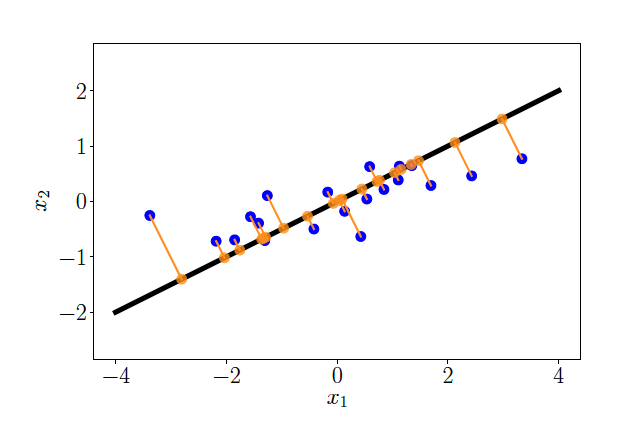
\includegraphics[width=0.7 \textwidth]{sections/images/orth1.png}

\textbf{Orthogonal projection onto a subspace of dimension 1.} 

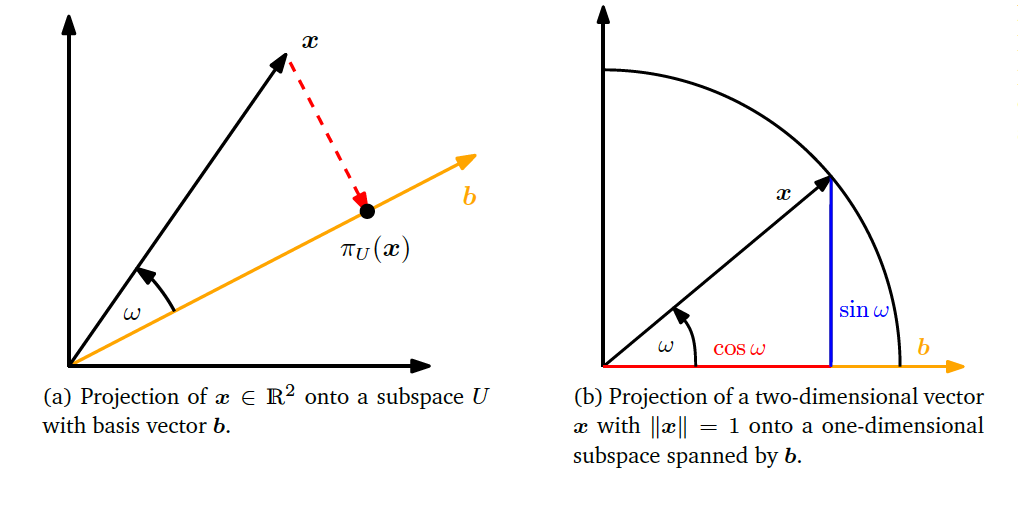
\includegraphics[width=0.7 \textwidth]{sections/images/orth2.png}

\begin{itemize}
    \item The projection $z=\Pi_U(\vec{x})$ is the closest point to $\vec{x}$ of the subspace $U$ generated by $\vec{b}$  by considering as the measure of the distance the 2-norm ($\| \cdot \|_2$). The vector $\zz -\xx$ (the red dashed one in the figure) is orthogonal to the subspace $U$ (and to the vector $\bb$ generating $U$). Hence, the scalar product: $<\vec{z}-\vec{x},\vec{b}>=0$
    \item The vector $\vec{z}$ is a vector of the subspace generated by $\vec{b}$, hence $\vec{z}=\alpha \vec{b}$, $\alpha \in \mathbf{R}.$
  
\end{itemize}


%\begin{example} (In 2 dimensions)\\
    % Let $\vec{y} \in \set{R}^2$ and $L=\text{span}\{\vec{u}\}$ one-dimensional subspace of $\set{R}^2$ generated by $\vec{u} \in \set{R}^2$. We can write $\vec{y}$ as
    % $$ \vec{y} = \hat{\vec{y}} + \vec{z} $$
    % and notice that $\vec{u} \parallel \hat{\vec{y}}$.
    
    % The projection $\hat{\vec{y}}$ is the closest vector lying in the subspace $L$ to $\vec{y}$, where distance is measured by $\norm{\vec{y} - \hat{\vec{y}}}$. It follows that $\vec{z} = \vec{y} - \hat{\vec{y}}$ is orthogonal to $L$ and, in particular, to $\vec{u}$, i.e. $\langle\vec{z}, \vec{u}\rangle = 0$.
    
   % Since $\hat{\vec{y}}$ is an element of $L$ it is a multiple of $\vec{u}$
    %$$ \hat{\vec{y}} = \alpha\vec{u} $$
    
    We can find $\alpha$ in the following way
    $$ \langle\vec{x} - \zz, \vec{b}\rangle = 0 \implies \langle\vec{z} - \alpha\vec{x}, \vec{b}\rangle = 0 \implies \langle\vec{x}, \vec{b}\rangle - \alpha\langle\vec{b}, \vec{b}\rangle = 0 $$
    $$ \alpha = \frac{\langle\vec{x}, \vec{b}\rangle}{\langle\vec{b}, \vec{b}\rangle} = \frac{\transp{\vec{x}}\vec{b}}{\norm{\vec{b}}^2} $$
%\end{example}

Example when projecting from $\mathbf{R}^3$ to $\mathbf{R}^2$.

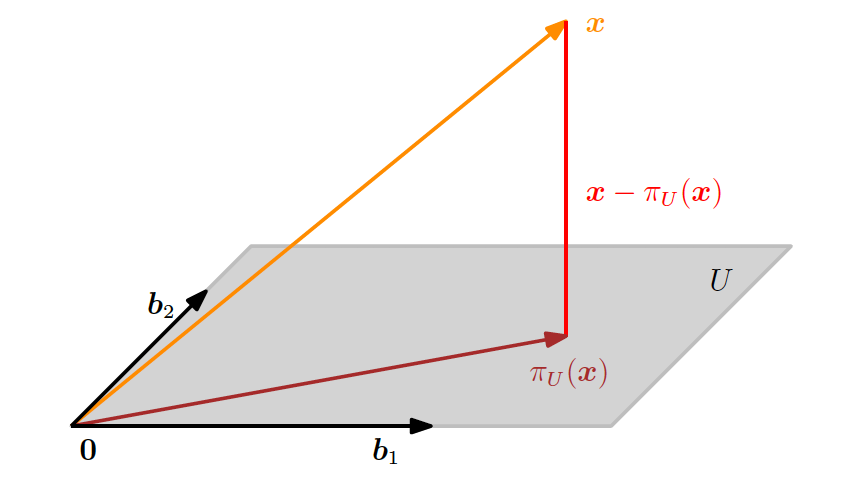
\includegraphics[width=0.7 \textwidth]{sections/images/orth3.png}

We now generalize to sub-spaces of dimension possibly greater than one.

\begin{theorem} (Best approximation theorem)
    Let $W$ a subspace with dimension $p$ of $\set{R}^n$, $\vec{y} \in \set{R}^n$ and $\hat{\vec{y}} = \mathrm{proj}_W(\vec{y})$. Then $\norm{\vec{y} - \hat{\vec{y}}} < \norm{\vec{y} - \vec{v}},\ \forall \vec{v} \in W,\ \vec{v} \neq \hat{\vec{y}}$.
\end{theorem}

This means that $\hat{\vec{y}}$ is the best approximation of $\vec{y}$ in $W$.

Example 3.10 MML book.

The idea is to use projections to find the vector in $\text{Col}(\mat{A})$ (i.e. the subspace generated by set of all the columns of $\AAA$) which is closest to $\vec{b}$. As already seen in the previous chapter, this vector is indeed the orthogonal projection of $\vec{b}$ onto the subspace $\text{Col}(\mat{A})$.

\subsubsection{The linear least squares problem}

When $\AAA$ has size $m \times n$ with $m>n$, it is not possible to find a solution of the linear system $\AAA \xx=\bb$.
The orthogonal projections allow to find a vector $\xx$ that is \textit{near} the system solution (in the sense of the 2-norm).

The problems is then formulated as to compute 
 $\hat{\xx}$ so that:
\begin{equation}
   \hat{\xx}= argmin_x \|\AAA \xx-\bb\|_2^2
   \label{llsq}
\end{equation}

For what concerns existence and uniqueness of the solution of the linear least squares problem, 
two different cases are possible:

\begin{itemize}
    \item $\rank{A} = n$, meaning that every column of $\mat{A}$ is linearly independent. A unique solution exists $\forall \vec{b} \in \set{R}^m$. Let $\vec{x^{*}}$ be the approximate solution to the linear system, we have
    $$ \mat{A}\vec{x^{*}} = \text{proj}_{\text{Col}(\mat{A})}(\vec{b}) $$
    This means that
    $$ \vec{b} - \mat{A}\vec{x^{*}} \in [\text{Col}(\mat{A})]^{\perp} \implies \transp{A}(\vec{b} - \mat{A}\vec{x^{*}}) = 0 $$
    Thus, we obtain the \textit{normal equations}
    $$ \transp{A}\mat{A}\vec{x^{*}} = \transp{A}\vec{b} $$
    which is a linear system in $n$ equations and $n$ unknowns. $\transp{A}\mat{A}$ is called \textit{Gramian matrix} of $\mat{A}$ and is non-singular, positive definite and symmetric. The approximate solution can then be obtained
    $$ \vec{x^{*}} = \inv{(\transp{A}\mat{A})}\transp{A}\vec{b} $$
    \item $\rank{A} = k,\ k < n$, meaning that there is an infinite number of solutions ($\infty^{n-k}$). We can find the least squares solution to the problem by using the pseudoinverse of $\mat{A}$ obtained via SVD
    $$ \mat{A}\vec{x} = \vec{b} \implies \mat{A}^{+}\mat{A}\vec{x^{*}} = \mat{A}^{+}\vec{b} \implies \vec{x^{*}} = \mat{A}^{+}\vec{b} \implies \vec{x^{*}} = \sum_{i=1}^{k}{\frac{\transp{\vec{u}_i}\vec{b}}{\sigma_i}\vec{v}_i} $$
\end{itemize}

It is possible to modify the linear least squares problem \eqref{llsq}  by introducing a weight matrix with the aim to give different weights to the components of $\xx$. 
\begin{equation}
   \hat{\xx}= argmin_x \|\vec{W} \AA \xx-\bb\|_2^2
   \label{wllsq}
\end{equation}
where $\vec{W}$ is an invertible matrix. In this case the \textit{weighted normal equations} are:
$$(\mat{W}\AAA)^T\mat{W}\AAA \xx=(\mat{W}\AAA)^T \bb$$


